\documentclass[a4paper,13.6pt]{article}
\usepackage{listings}
\usepackage{CJKutf8}
\usepackage{minted}
\usepackage{picinpar,graphicx}
\usepackage[utf8]{inputenc}
\usepackage[T1]{fontenc}
\usepackage{CJK}
\usepackage{geometry}
\author{Weiers\&IronHead}
\title{ACM-template}
\usepackage{lastpage}%获得总页数
\usepackage{fancyhdr}
\usepackage{pdfpages}
\usepackage[colorlinks,linkcolor=black]{hyperref}
\pagestyle{fancy}
%以下命令中L--左侧 R--右侧 C--中间 O--奇数页 E--偶数页
\fancyhead[LO,RE]{ACM-template}%奇数页左侧,偶数页右侧显示页眉
\fancyfoot[CO,RE]{I LOVE ACM!}%奇数页中间,偶数页右侧页脚为空
\fancyfoot[LO,CE]{}%奇数页左侧,偶数页中间页脚为空
\fancyfoot[RO,LE]{\thepage\ of
\pageref{LastPage}}%奇数页右侧,偶数页左侧显示 当前页 of 总页数
\renewcommand{\headrulewidth}{0.4pt}%改为0pt即可去掉页眉下面的横线
\renewcommand{\footrulewidth}{0.4pt}
\geometry{left = 2.5cm,right = 2.5cm,top = 2.5cm,botton = 2.5cm}
\begin{document}
\maketitle
\vspace{3cm}
\begin{CJK}{UTF8}{gbsn}
    
\newpage

\tableofcontents
\newpage

\section{头文件}
\inputminted{c++}{../ACM_Template/Others/Include.cpp}
\newpage
\section{图论}
\subsection{最短路}
\inputminted{c++}{../ACM_Template/Graph/Shortest_Path.cpp}
\subsection{最小生成树}
\inputminted{c++}{../ACM_Template/Graph/Minimal_Spanning_Tree.cpp}
\subsection{二分图}
\inputminted{c++}{../ACM_Template/Graph/Bipartite_Graph_Matching.cpp}
\subsection{2-SAT}
\inputminted{c++}{../ACM_Template/Graph/2-SAT.cpp}
\subsection{割点与强连通}
\inputminted{c++}{../ACM_Template/Graph/Strongly_Connected_Component.cpp}
\subsection{最大流}
\inputminted{c++}{../ACM_Template/Graph/Network_Flow.cpp}
\subsection{最小费用最大流}
\inputminted{c++}{../ACM_Template/Graph/MinCost_MaxFlow.cpp}
\subsection{第k短路}
\inputminted{c++}{../ACM_Template/Graph/The_K_Shortest_Path.cpp}
\subsection{欧拉路径}
\inputminted{c++}{../ACM_Template/Graph/Eular_Path.cpp}
\subsection{次小生成树}
\inputminted{c++}{../ACM_Template/Graph/Second_Minimal_Spanning_Tree.cpp}
\newpage

\section{数据结构}
\subsection{并查集}
\inputminted{c++}{../ACM_Template/Data_Structure/Union-Find_Set.cpp}
\subsection{LCA}
\inputminted{c++}{../ACM_Template/Data_Structure/LCA.cpp}
\subsection{RMQ}
\inputminted{c++}{../ACM_Template/Data_Structure/RMQ.cpp}
\subsection{线段树}
\inputminted{c++}{../ACM_Template/Data_Structure/Segment_Tree.cpp}
\subsection{树状数组}
\inputminted{c++}{../ACM_Template/Data_Structure/Binary_Indexed_Tree.cpp}
\subsection{主席树}
\inputminted{c++}{../ACM_Template/Data_Structure/Functional_Segment_Tree.cpp}
\subsection{树链剖分}
\inputminted{c++}{../ACM_Template/Data_Structure/Heavy-Light_Decomposition.cpp}
\subsection{LCT}
\inputminted{c++}{../ACM_Template/Data_Structure/LCT.cpp}
\subsection{Splay}
\inputminted{c++}{../ACM_Template/Data_Structure/Splay.cpp}
\subsection{区间不同数}
\inputminted{c++}{../ACM_Template/Data_Structure/Different_Numbers_Of_Interval.cpp}
\subsection{矩形面积并}
\inputminted{c++}{../ACM_Template/Data_Structure/Area_And.cpp}
\subsection{矩形面积交}
\inputminted{c++}{../ACM_Template/Data_Structure/Area_cross.cpp}
\subsection{矩形周长并}
\inputminted{c++}{../ACM_Template/Data_Structure/Perimeter_And.cpp}
\newpage

\section{字符串}
\subsection{哈希}
\inputminted{c++}{../ACM_Template/String/Hash.cpp}
\subsection{KMP}
\inputminted{c++}{../ACM_Template/String/KMP.cpp}
\subsection{扩展KMP}
\inputminted{c++}{../ACM_Template/String/Exkmp.cpp}
\subsection{Manacher}
\inputminted{c++}{../ACM_Template/String/Manacher.cpp}
\subsection{01字典树}
\inputminted{c++}{../ACM_Template/String/01Trie.cpp}
\subsection{ac自动机}
\inputminted{c++}{../ACM_Template/String/Aho-Corasick_Automaton.cpp}
\subsection{后缀数组}
\inputminted{c++}{../ACM_Template/String/Suffix_Array.cpp}
\subsection{后缀自动机}
\inputminted{c++}{../ACM_Template/String/Suffix_Automation.cpp}
\subsection{回文自动机}
\inputminted{c++}{../ACM_Template/String/Palindrome_Automata.cpp}

\newpage
\section{优化算法}
\subsection{二分}
\inputminted{c++}{../ACM_Template/Optimize/Binary_Search.cpp}
\subsection{数位DP}
\inputminted{c++}{../ACM_Template/Optimize/Digit_Statistics.cpp}
\subsection{树上启发式合并}
\inputminted{c++}{../ACM_Template/Optimize/DSU_On_Tree.cpp}
\subsection{莫队算法}
\inputminted{c++}{../ACM_Template/Optimize/Mo_Algorithm.cpp}
\subsection{单调栈单调队列笛卡尔树}
\inputminted{c++}{../ACM_Template/Optimize/Monotone_Stack_Queue_Tree.cpp}
\subsection{最长上升子序列}
\inputminted{c++}{../ACM_Template/Optimize/The_Longest_Increasing_Subsequence.cpp}

\newpage
\section{不会数学}
\subsection{快速幂与矩阵快速幂}
\inputminted{c++}{../ACM_Template/Math/Fast_Power.cpp}
\subsection{欧几里得与逆元}
\inputminted{c++}{../ACM_Template/Math/Euclid_And_Inverse.cpp}
\subsection{欧拉函数}
\inputminted{c++}{../ACM_Template/Math/Eular_phi.cpp}
\subsection{素数与质因子}
\inputminted{c++}{../ACM_Template/Math/Primes_And_Factors.cpp}
\subsection{组合数学与容斥原理}
\inputminted{c++}{../ACM_Template/Math/CombinatoricsMath_And_Exclusion.cpp}
\subsection{中国剩余定理}
\inputminted{c++}{../ACM_Template/Math/China_Remainder_Theorem.cpp}
\subsection{FFT}
\inputminted{c++}{../ACM_Template/Math/FFT.cpp}

\newpage
\section{各种操作}
\subsection{二进制位操作} 
\begin{itemize}
\item \_\_builtin\_ffs(x)  返回x中最后一个为1的位是从后向前的第几位,从1开始计数

\item \_\_builtin\_popcount(x)  x中1的个数。

\item \_\_builtin\_ctz(x)  x末尾0的个数。x=0时结果未定义。

\item \_\_builtin\_clz(x)  x前导0的个数。x=0时结果未定义。

上面的x都是unsigned int型的,如果传入signed或者是char型,会被强制转换成unsigned int

\item \_\_builtin\_parity(x)  x中1的个数的奇偶性,返回1为奇。
\end{itemize}

\subsection{bitset} 
\begin{itemize}
\item bitset<100000>bt;
\item bt<<1; //整体移位
\item bt|=10;
\item bt.count(); //b中置为1的二进制位的个数
\item bt.size(); //b中二进制位的个数
\item bt[pos]; //访问b中在pos处的二进制位
\item bt.test(pos); //b中在pos处的二进制位是否为1
\item bt.set(); //把b中所有二进制位都置为1
\item bt.set(pos); //把b中在pos处的二进制位置为1
\item bt.reset(); //把b中所有二进制位都置为0
\item bt.reset(pos); //把b中在pos处的二进制位置为0
\end{itemize}

\subsection{nth\_element} 
\begin{itemize}
\item nth\_element(first,nth,last)
\item first,last 第一个和最后一个元素位置
\item nth:要定位的第n个元素
\item nth\_element会将第n\_th 元素放到它该放的位置上,左边元素都小于它,右边元素都大于它
\item 期望复杂度o(n)
\item  nth\_element(a,a+6,a+10)
\end{itemize}

\subsection{Rope} 
\inputminted{c++}{../ACM_Template/Operation/gnu_rope.cpp}

\subsection{pb\_ds} 
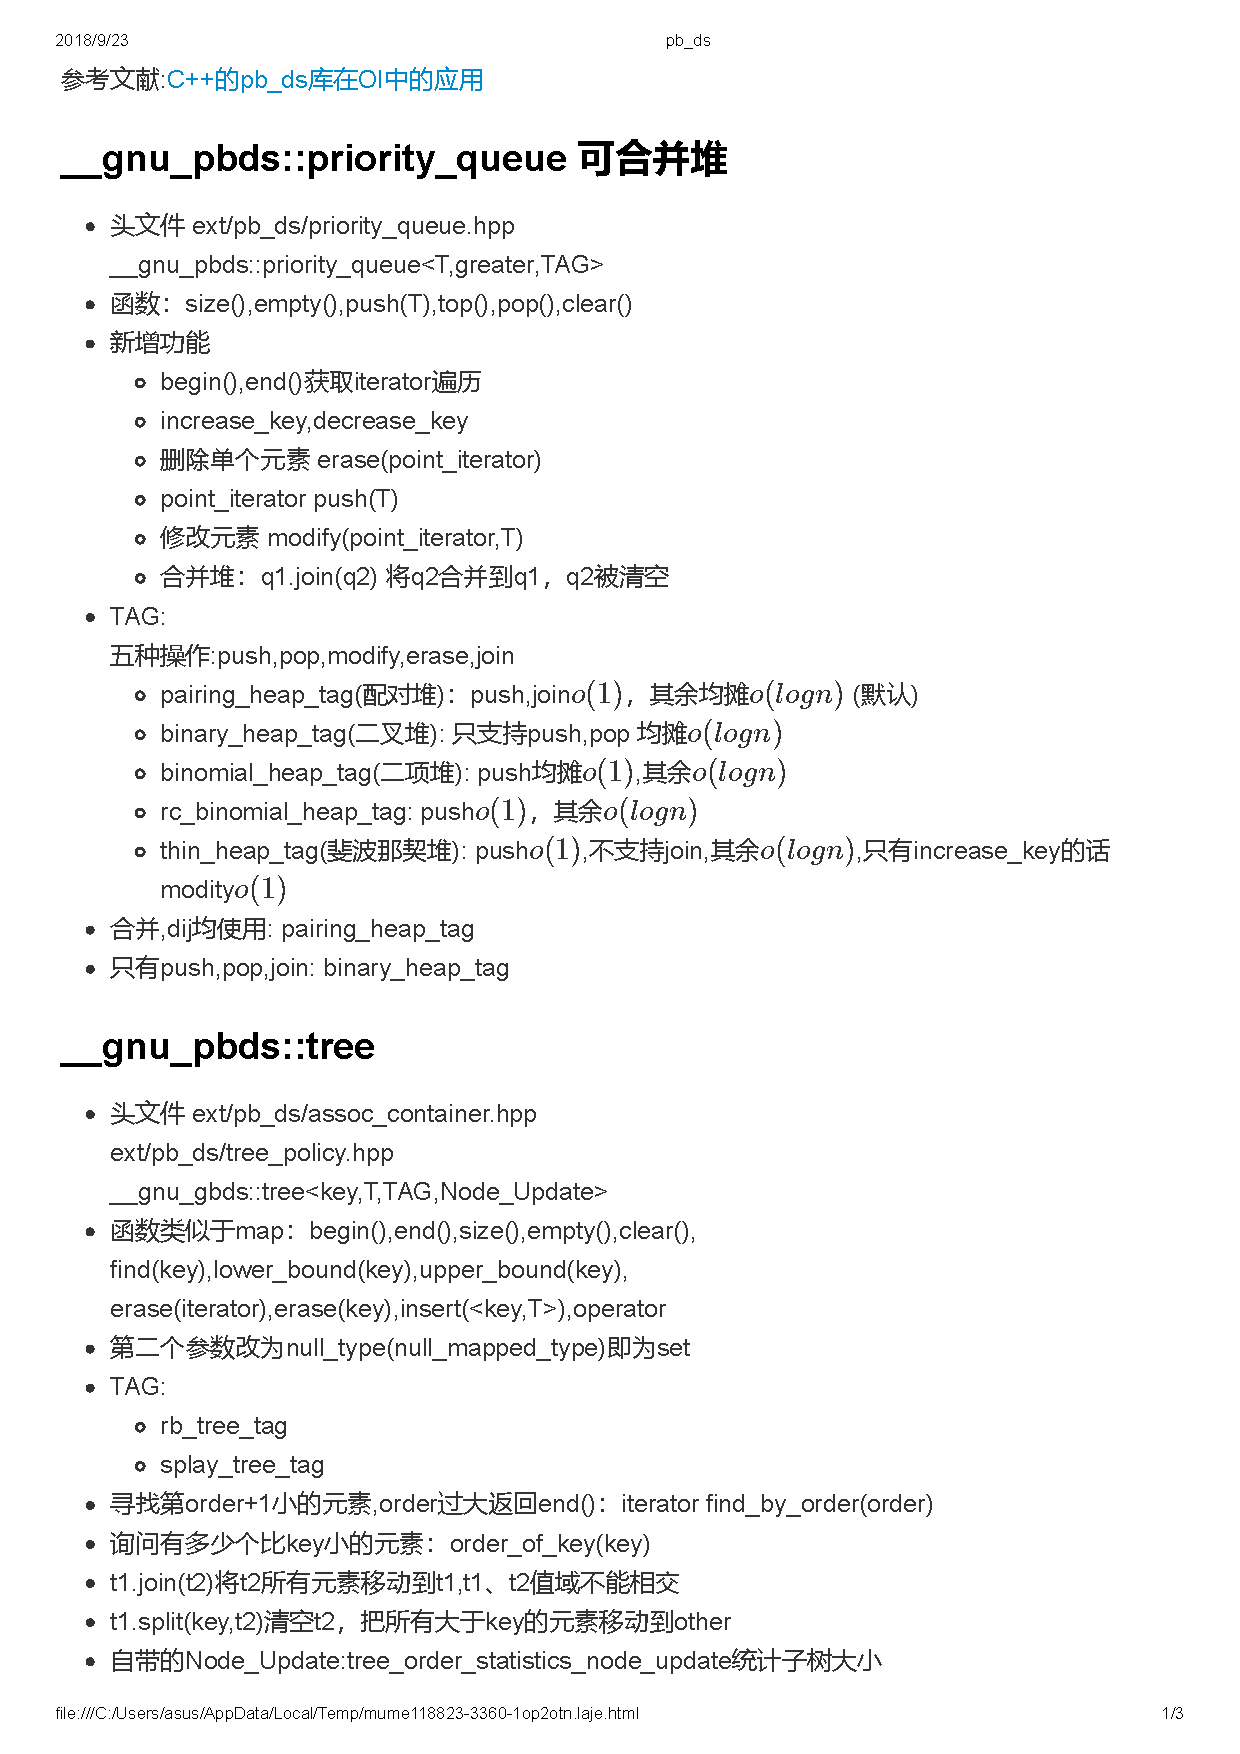
\includepdf[pages=1-2,offset=0cm 0.5cm]{../ACM_Template/Operation/pb_ds.pdf}

\subsection{String And Char}
\inputminted{c++}{../ACM_Template/Operation/StringAndChar.cpp}

\subsection{String To Int}
\subsubsection*{int/float to string/array}
\begin{itemize}
\item itoa():将整型值转换为字符串。
\item ltoa():将长整型值转换为字符串。
\item ultoa():将无符号长整型值转换为字符串。
\item gcvt():将浮点型数转换为字符串,取四舍五入。
\item ecvt():将双精度浮点型值转换为字符串,转换结果中不包含十进制小数点。
\item fcvt():指定位数为转换精度,其余同ecvt()。
\end{itemize}

\subsubsection*{string/array to int/float}
\begin{itemize}
\item atof():将字符串转换为双精度浮点型值。
\item atoi():将字符串转换为整型值。
\item atol():将字符串转换为长整型值。
\item strtod():将字符串转换为双精度浮点型值,并报告不能被转换的所有剩余数字。
\item strtol():将字符串转换为长整值,并报告不能被转换的所有剩余数字。
\item strtoul():将字符串转换为无符号长整型值,并报告不能被转换的所有剩余数字。
\end{itemize}


\subsection{IO}
\inputminted{c++}{../ACM_Template/Operation/IOgetchar.cpp}

\inputminted{c++}{../ACM_Template/Operation/Short_IO.cpp}

\subsection{Other Tips}
\inputminted{c++}{../ACM_Template/Operation/tips.cpp}

\newpage
\section{Java}
\subsection{高精度}
\inputminted{java}{../ACM_Template/Java/BigDecimal.java}
\subsection{Java输入输出}
\inputminted{java}{../ACM_Template/Java/Java_input_output.java}
\subsection{Java快速读入}
\inputminted{java}{../ACM_Template/Java/javafastin.java}


\newpage
嘤嘤嘤
\end{CJK}
\end{document}
